\chapter{Tools of Radio Astronomy}

Radio astronomy found its beginning at Bell labs, Karl Janksy announced in 1933 the discovery radio emission coming from the Milky Way when observing the atmosphere at 20~MHz \citep{jansky_radio_1933}. This was soon improved upon by Grote Reber, who built a radio telescope in his backyard and made deliberate observations of many radio bright objects, publishing them in astronomical journals. Radio transmitters and receivers made great strides during the war years due to the development of radar equipment for military purposes. In the following years many who had developed these technologies, turned to study the `noise' that was picked up from extraterrestrial sources, forming the foundation of modern radio astronomy. 

The radio window from the Earth's surface extends roughly from 30~MHz $(\lambda\sim10~\mathrm{m})$ up to about 1300~GHz $(\lambda\sim0.3~\mathrm{mm})$ as shown in \cref{fig:chpt2radiowindow}. The lower limit of this window arises from adsorption of radio waves by free electrons in the ionosphere. While radio waves can technically be observed down to 4.5~MHz if the frequency of the radio waves is below that of the plasma frequency, $\nu_p$ the adsorption becomes significantly more prominent such that

\begin{equation}
    \frac{\nu_P}{\mathrm{kHz}} = 8.97 \sqrt{\dfrac{N_e}{\mathrm{cm^{-3}}}}, 
\end{equation}

Where $N_e$ is the electron density of the plasma. There is also other contributions that effect this, such as solar activity which make this limit variable. This means that to study kHz frequencies or an unrefracted view of $\lesssim 30~\mathrm{MHz}$ the radio sky must be observed from space. The upper radio limit isn't observed at any single wavelength, but considerations become important at mm wavelengths as resonant absorption comes into effect from the lowest rotation band of molecules in the troposphere \citep{WilsonToolsofRadioastron}. This is mainly attributed to water vapour $\mathrm{H}_2\mathrm{O}$ and $\mathrm{O_2}$, adsorption also occurs at higher frequencies, but here the atmosphere is opaque to radio waves. Around 300~GHz is considered to the upper limit in a radio context where atmospheric absorption at sea level becomes very strong, with additional losses from clouds and rain. The work in this thesis is carried out from $0.1-4000~\mathrm{MHz}$. 

This chapter discusses some fundamentals of radio telescopes and the processes that go into generating science useable products used to explore the objects discussed in \cref{chap:introduction}.

\begin{figure}
    \centering
    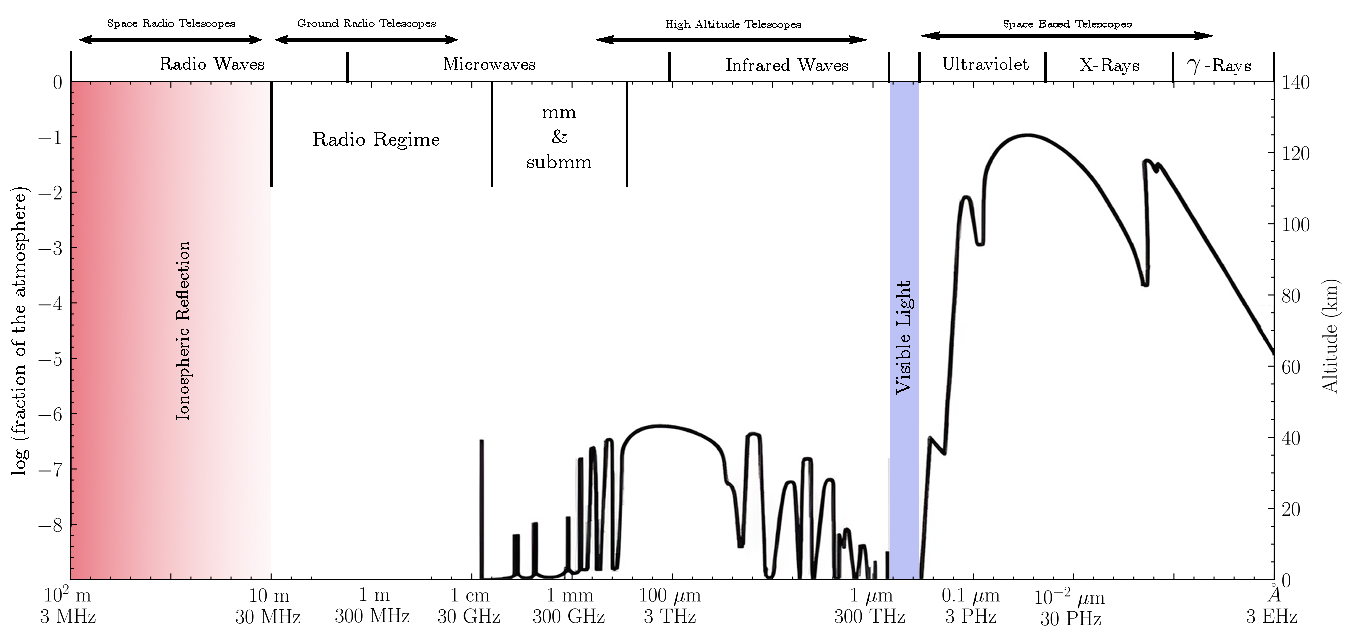
\includegraphics[width=0.98\linewidth]{chapter2/figures/atmospheric_reflection_render.pdf}
    \caption{Atmospheric attenuation as a function of wavelength and frequency. Values are taken to reflect when the incoming radiation has been attenuated by a factor of 1/2. Figure adapted from \cite{WilsonToolsofRadioastron}}
    \label{fig:chpt2radiowindow}
\end{figure}

\section{From Photon to Filterbank}

Radio telescopes can often be seen as conceptually complex but share much common ground with contemporary optical telescopes. An antenna is often thought of as a `single pixel' in a charged couple device (CCD) with an array of antennas forming an array of pixels that can be used to observe the sky. There are also parallels to be drawn between the mirrors in optical telescope and the parabolic dishes seen on radio telescopes which will later be discussed. This section aims to provide enough theoretical context to understand how an incident photon on a radio telescope gets turned into science useable data products such as filterbanks. 

For any electromagnetic wave coming from an astronomical source the wave is considered to be in the far-field, and the wavefronts are therefore locally planar across the extent of a radio telescope. Radio telescopes sample the electric field associated with these incoming plane waves. The general time-dependent electric field vector may be expressed as,

\begin{equation}
    \textbf{E} (t,r) = (\hat a E_a + \hat b E_b) \ \exp(2 \pi i (ft-kr))
    \label{eq:wave_equation}
\end{equation}

%TODO: talk about r_1, r_2, phase difference for interferometry down the line. Add references to the books used to come up with these derivations 

where $\hat a$ and $\hat b$ are orthogonal polarisation basis vectors, $z$ is the orthogonal axis which the wave progates forward with time, $t$. $E_a$ and $E_b$ are the corresponding complex amplitudes, $f$ is wave frequency, $k$ is the wavenumber, $2 \pi \lambda$. 
In short, in \cref{eq:wave_equation} the first term dictates the wave polarisation and the second term dictates the wave propagation. If a radio telescope samples the plane wave at a given instant, the polarisation term\footnote{Independent of the propagation term and associated phase.} can be described by a Jones vector, 

\begin{equation}
   \mathbf{j}
    =
    \begin{pmatrix}
        E_a \\ 
        E_b
    \end{pmatrix}
    =
    E_0 
    \begin{pmatrix}
        \cos\psi \cos\beta - i\sin\psi \sin\beta \\
        \sin\psi \cos\beta + i\cos\psi \sin\beta
    \end{pmatrix}.
    \label{eq:chap2jonesvector}
\end{equation}

Here, $\beta$ describes the shape and `handness' of the ellipse that is traced out by the wave vector, shown in \cref{fig:chpt2planewavepol}, which is what the radio telescope `sees' when it samples the wave depending on the value of $\beta$. When $\beta$ is $90^\circ$ or $0^\circ$ the wave has a linear polarisation, $\beta = \pm 45$ gives a fully circularised, with $+$ denoted has `right handed' and $-$ as `left handed'. Any other values of $\beta$ will produce elliptical traces. Varying $\psi$ in this case the polarization ellipse but doesn't changing its shape.

\begin{figure}
    \centering
    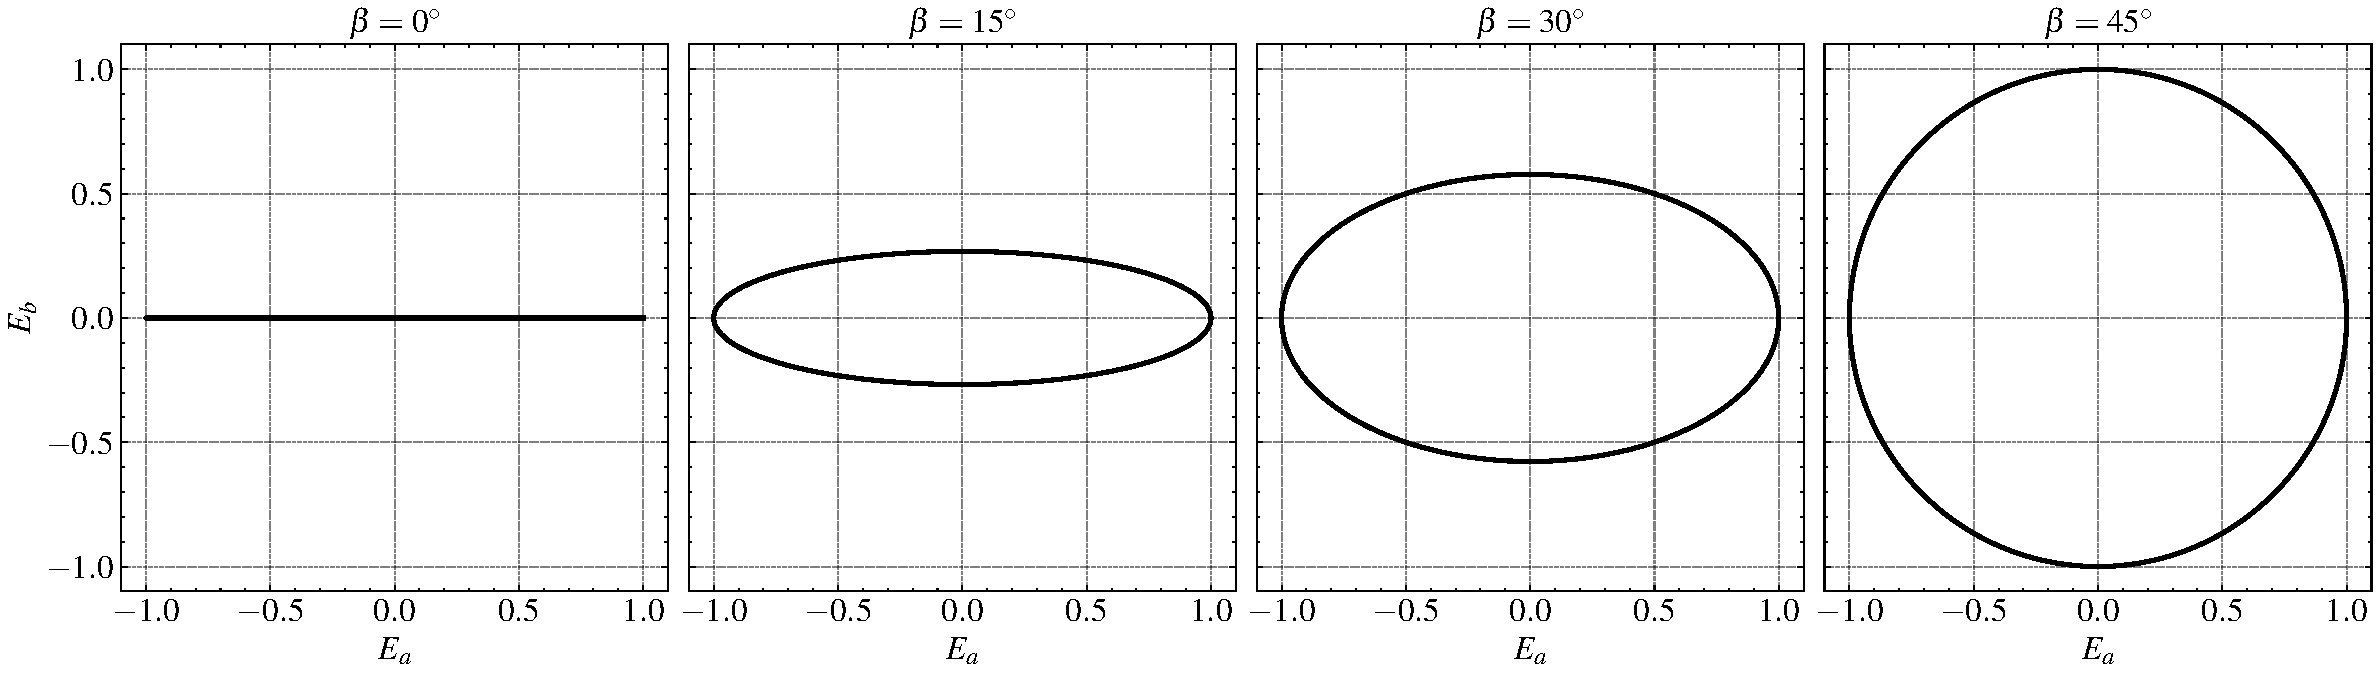
\includegraphics[width=0.98\linewidth]{chapter2/figures/plane_wave_polarization.pdf}
    \caption{The real ($\mathcal{R}$) values of the plane wave equation $a$ and $b$ components for different values of $\beta$.}
    \label{fig:chpt2planewavepol}
\end{figure}

As an instantaneous wave plane isn't observable a time averaged representation that contains observables needs to be expressed. Taking the outer product of the Jones vector with its Hermitian transpose and taking a time average yields the coherency matrix \citep{hamaker_understanding_1996} which is expressed as follows, 

\begin{equation}
\mathbf{J}
=
\left\langle
\mathbf{j}\mathbf{j}^{\dagger}
\right\rangle
=
\begin{pmatrix}
\langle E_a E_a^{*} \rangle &
\langle E_a E_b^{*} \rangle \\
\langle E_b E_a^{*} \rangle &
\langle E_b E_b^{*} \rangle
\end{pmatrix}
=
\frac{1}{2}
\begin{pmatrix}
I + Q & U + iV \\
U - iV & I - Q
\end{pmatrix}, 
\label{eq:chap2cohermatrix}
\end{equation}

The elements can of the coherency matrix can expressed in terms of the four Stokes parameters \citep{stokes_xxx_1852}. The Stokes parameters provide an observable relation to describe polarised light which are extensively used in radio astronomy usually in the following form. 

\begin{align}
I \equiv  & E^2 = E^2_x + E^2_y,\\ 
Q \equiv & I \cos 2\psi \ \cos 2\beta = E^2_x - E^2_y,\\
U \equiv  & I \sin 2\psi \ \cos 2\beta = 2 E_x E_y \cos 2 \phi,\\
V \equiv & I \sin 2\beta = 2 E_x E_y \sin \phi.
\end{align}

Radio telescopes only measure $x$ and $y$ in the electric field plane $(E_x,E_y)$. $\psi$ is the rotation of the wave in respect to the plane of the ellipse \citep[][p. 261]{pulsar_handbook}.